\begin{figure*}[t]
     \centering
     \begin{subfigure}[b]{0.32\textwidth}
         \centering
         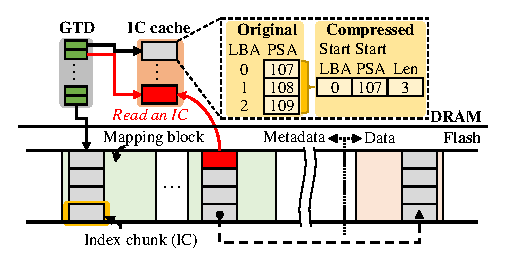
\includegraphics[width=\textwidth]{figs/OSDI/koo/dftl.eps}
         %\vspace{-5pt}
         \caption{Demand-based indexing}
         %\caption{Hybrid indexing (FAST~\cite{fast})}
         \label{fig:demand}
     \end{subfigure}
     \hfill
     \begin{subfigure}[b]{0.32\textwidth}
         \centering
         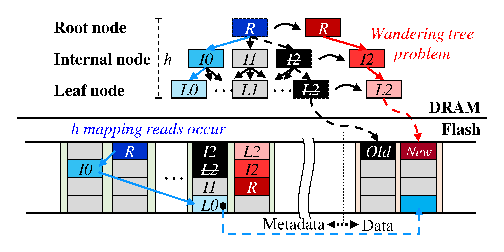
\includegraphics[width=\textwidth]{figs/OSDI/koo/uftl.eps}
         %\vspace{-5pt}
         \caption{Tree-based indexing ($\mu$-FTL~\cite{uftl})}
         \label{fig:mutree}
     \end{subfigure}
     \hfill
     \begin{subfigure}[b]{0.32\textwidth}
         \centering
         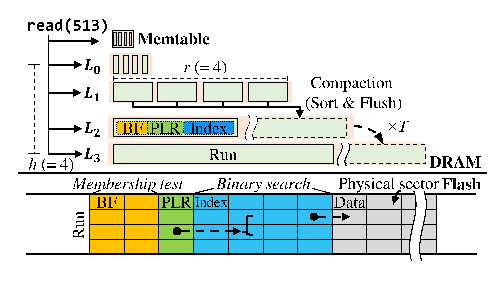
\includegraphics[width=\textwidth]{figs/OSDI/koo/lsm-short.eps}
         %\vspace{-5pt}
         \caption{LSM-tree indexing}
         \label{fig:LSM-tree}
     \end{subfigure}
    \vspace{-5pt}
	 \caption{Index structures for SSDs}
    \vspace{-20pt}
    \label{fig:ftl-review}
\label{fig:back-idx}
\end{figure*}





\begin{figure}[t]
     \centering
     \begin{subfigure}[b]{0.228\textwidth}
         \centering
         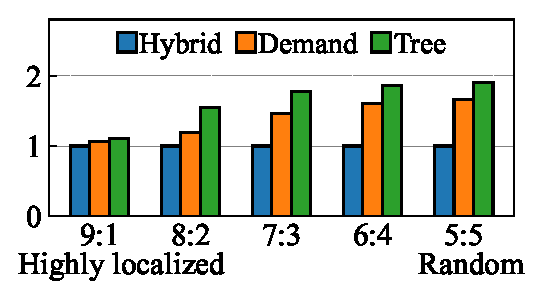
\includegraphics[width=\textwidth]{figs/OSDI/new-simul-raf.eps}
         %\vspace{-10pt}
         \caption{RAF}
        \vspace{-10pt}
     \end{subfigure}
     \hfill
     \begin{subfigure}[b]{0.24\textwidth}
         \centering
         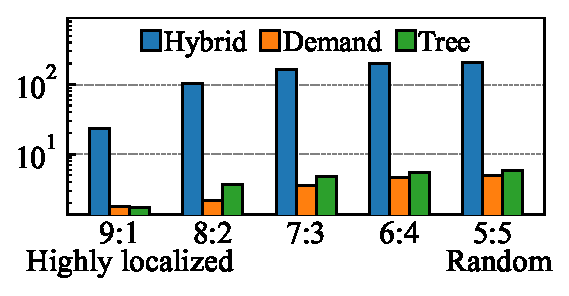
\includegraphics[width=\textwidth]{figs/OSDI/new-simul-waf.eps}
         %\vspace{-10pt}
         \caption{WAF}
         \vspace{-10pt}
         \end{subfigure}
	 \caption{Simulation results of three index structures}
\label{fig:simul-result}
\end{figure}

\begin{comment}
\begin{figure*}[t]
\centering
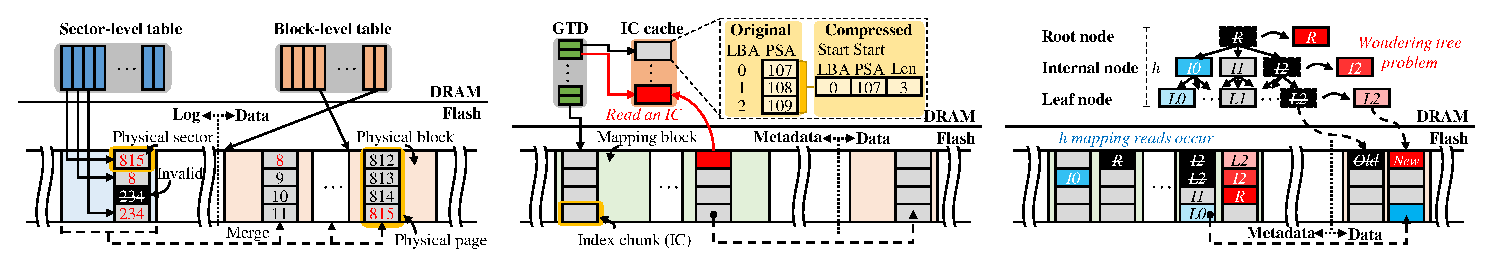
\includegraphics[height=2.85cm]{figs/OSDI/new_figs.eps}
\vspace{-3pt}
\caption{\koo{Indexing structures for SSDs}}
\label{fig:existing}
\vspace{-12pt}
\end{figure*}
\end{comment}

%-----------------------------------------------------------------------------
\section{Background and Related Work}
\label{sec:back}

We review existing index structures for SSDs 
that have been proposed over the past 20 years and 
discuss their limitations.  
%We focus on evaluating two important factors,
%a read amplification factor (RAF) and a write amplification factor (WAF),
%which represent how many \koo{\st{extra} flash} I/Os occur 
%while handling \koo{user-requested} I/Os.

\subsection{NAND Flash Basics}
\label{sec:back:table}

A NAND flash is composed of blocks, each of which consists of 128$\sim$256
pages, typically 16KB in size.  While a page is the unit of reads and
writes, a block is the unit of erasure. A 16KB page is larger than a 4KB
logical block that is the unit of I/Os in the host. Thus, four logical blocks
are stored together in the same page in a 4KB physical sector unit.  Each page
has an out-of-band (OOB) area to keep metadata (\ie~logical block
addresses) associated with the data. 

To hide the unusual property of NAND flash that does not support in-place
updates, SSD firmware, called a flash translation layer (FTL), 
appends incoming
data to free space in the flash.  
Suppose that data for a logical block address
(LBA) \LBA{i} was written to a physical sector address (PSA) \PSA{i}.
If the data for \LBA{i} is modified, its up-to-date data must be
redirected to a free physical sector address \PSA{j}.  To keep track of the
physical locations of \LBA{i}, 
the FTL maintains a sector-level L2P table in DRAM. 
The table is indexed by \LBA{i}, 
and each entry locates a sector \PSA{j} where
\LBA{i}'s data is stored.
As SSD capacity gets larger, keeping the index table entirely in DRAM becomes
difficult.  To reduce DRAM requirement, many have proposed various index
structures.

\subsection{Existing Index Structures for SSDs}
Existing index structures are categorized into three types: 
hybrid~\cite{fast,superblockFTL, last, flexibleFTL}, 
tree-based~\cite{ubifs,uftl,utree}, and demand-based
indexing~\cite{dftl,sftl,tpftl}.
We focus on evaluating two important factors,
a read amplification factor (RAF) and a write amplification factor (WAF),
which represent how many flash I/Os occur 
while handling user-requested I/Os.
\TAB{tab:raf-cost} summarizes the RAFs of the index structures.
We also conduct a simulation study using synthetic workloads with
different locality to compare RAFs and WAFs of different indexing techniques.
%understand their performance characteristics.
For the simulation, we use an SSD emulator with 512GB capacity.
A page size is 16KB and the number of pages per block is 128.
Our results are depicted in \FIG{fig:simul-result}.

\textbf{Hybrid Indexing.}
Hybrid indexing uses sector- and (flash) block-level indices to alleviate memory
pressure~\cite{fast,superblockFTL, last, flexibleFTL}.  
It splits an SSD space into log and data areas. 	
Incoming data is first written to the log area
managed by a sector-level table.
Once the log area becomes full, valid data in the log is evicted to
(or merged with) blocks in the data area.
The data area is managed by a block-level table
that uses a coarse-grained index unit and is thus memory efficient.
The log area is set small,
and most of the SSD space is used for the data area.
The hybrid indexing guarantees RAF of 1.0
(see~\TAB{tab:raf-cost}).
This is possible because
both sector- and block-level tables can entirely reside in DRAM
owing to their small sizes.
Its biggest drawback is high WAF. Moving valid data 
in the log to the data area involves many
I/Os. According to our simulation, its WAF increases up to 209.68 
(see~\FIG{fig:simul-result}).
%For this reason, the hybrid indexing is not widely used today.

\textbf{Demand-based Indexing.}
Demand-based indexing is designed to leverage locality of I/O references to
save memory.  It divides an SSD space into metadata and data areas.
The entire L2P table is kept in the metadata area, 
while the data area stores user data (see \FIG{fig:ftl-review}(a)).  
The flash-resident table is split into
fixed-size index chunks (ICs), each of which is 4KB in size.
Only popular ICs with frequently referenced entries are cached in DRAM.  The
demand-based indexing maintains a global translation directory (GTD) that keeps
track of cached or flash-resident ICs.  
Some variants like SFTL~\cite{sftl} and DFTL~\cite{tpftl} 
try to cache more entries in DRAM
by delta-encoding entries pointing to physically
consecutive sectors.

The demand-based indexing provides RAF of 1.0 on a cache hit.
But, if a cache miss occurs, it has to fetch an IC from
the flash to DRAM. It involves one extra read, increasing RAF to 2.0.
The demand-based indexing thus has RAF $= 1 + \alpha_{miss}$,
where $\alpha_{miss}$ is a cache miss ratio.
As explained in \SEC{sec:intro}, 
its performance changes greatly
by workloads and storage fragmentation that affect a cache miss ratio.
%Its RAF is highly dependent upon a cache hit ratio,
%$\alpha_{hit}$: RAF = $1 + (1-\alpha_{hit})$. 
%\JS{이후 문장들 제거?}\todo{
To make in-memory metadata persistent, 
dirty ICs and corresponding GTD entries must be
immediately or regularly flushed out to the flash, which increases its WAF. 
%To
%mitigate this problem, some or all of them are backed up by capacitors 
%within an SSD controller~\cite{spartan}.}

%However, it often suffers from severe penalties.  When the desired entry is not
%found in the cache, it must be brought into DRAM on demand, which causes an
%extra read before serving a user request.  As a result, RAF of the demand-based
%indexing varies significantly according the degree of locality.  In the worst
%case, two extra reads are required to service a single read .  
%Moreover, if a dirty IC is chosen as a victim to evict, 
%corresponding GTD entries must be flushed out to the flash, which exacerbates
%overall WAFs. To mitigate the write amplification problem,
%the GTD is usually backed up by capacitors within an SSD controller.

\textbf{Tree-based Indexing.}
Some have attempted to use trees for indexing 
(see \FIG{fig:ftl-review}(b)).  The most well-known one is
$\mu$\--FTL~\cite{uftl} that uses a variant of a B+tree, $\mu$\--tree~\cite{utree}.
%In contrast to the demand-based indexing, the tree-based indexing keeps tree
%data structures in the metadata area.  
The tree-based indexing maintains three different types of nodes: a root node,
internal nodes, and leaf nodes.  The root and internal nodes have keys and
pointers to child nodes, and leaf nodes hold indices that locate data.
All the nodes are persisted in the metadata area of the flash,
but popular nodes are cached in DRAM like the demand-based one.  
The tree-based indexing 
indexes data in a variable-sized logical chunk unit. If logically
consecutive logical blocks are stored over physically continuous sectors, 
each index points to the start location of the chunk and its length.
This is similar to what SFTL and TPFTL do in the demand-based indexing.


%The tree-based indexing has relatively low lookup complexity, $O(log(n))$, and
%has a great potential to save DRAM by indexing data in a variable-sized chunk
%unit.  
While it seems effective, the tree-based indexing has several drawbacks. 
First, it suffers from the wandering tree problem~\cite{wandering-b+}.
%First, it suffers from the wandering tree problem that deteriorates
%both WAF and RAF~\cite{todo}.  
If new data is appended to the data area, 
then an associated leaf node, internal nodes, 
and even the root node must be
updated recursively (see red nodes in \FIG{fig:ftl-review}(b)). 
The updated nodes are
eventually written to the flash, increasing WAF. 
To retrieve an index of data to read, 
it has to traverse the root and internal nodes 
along the path to reach a
leaf node (see blue nodes in \FIG{fig:ftl-review}(b)). 
This may involve several reads, increasing RAF.
Second, 
%it is vulnerable to fragmentation. 
as storage space gets fragmented, logical chunks become smaller,
which generates many nodes.
This increases a tree height $h$, resulting in more memory consumption
and higher RAF.
Finally, it still
relies on caching, suffering from the same problem as the demand-based one.
Because of the aforementioned overheads,
the tree-based indexing has RAF = $1 + h \times \alpha_{miss}$
and performs poorer than the demand-based one (see~\FIG{fig:simul-result}).

\begin{comment}
\textbf{Simulation Result.}
\FIG{fig:simul-result} shows simulation results 
of the three indexing techniques under
synthetic workloads with different locality. We emualate
a \fixme{1TB SSD} where a flash page size is 16KB and the number of pages
per block is 128. The hybrid indexing exhibits the
lowest RAF, but suffers from the extremely high WAF owing to high merge costs.
Under localized workloads, the demand-based and table-based indexing perform
better than the hybrid indexing, exhibiting both fairly low RAF and WAF.
However, they show high RAF and WAF when an input workload has weak locality or
is random.  Owing to the wandering tree problem, the tree-based indexing cannot
outperform the demand-based one.
% Please add the following required packages to your document preamble:
% \usepackage{multirow}
\end{comment}
\begin{comment}
\begin{figure}[t]
     \centering
     \begin{subfigure}[b]{0.228\textwidth}
         \centering
         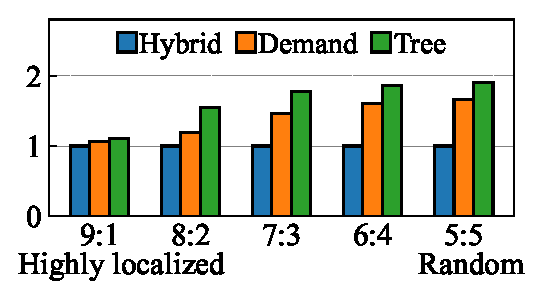
\includegraphics[width=\textwidth]{figs/OSDI/new-simul-raf.eps}
         \vspace{-10pt}
         \caption{RAF}
        \vspace{-10pt}
     \end{subfigure}
     \hfill
     \begin{subfigure}[b]{0.24\textwidth}
         \centering
         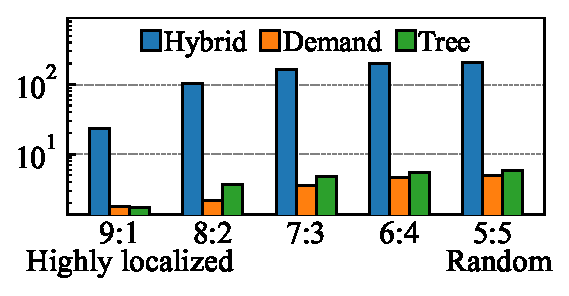
\includegraphics[width=\textwidth]{figs/OSDI/new-simul-waf.eps}
         \vspace{-10pt}
         \caption{WAF}
         \vspace{-10pt}
         \end{subfigure}
	 \caption{Simulation results of three index structures}
\label{fig:simul-result}
\end{figure}
\end{comment}

\begin{comment}

\textbf{LSM-tree-based Indexing.}
There exist some index designs that use a variant of LSM-trees in SSDs
(\eg~iLSM~\cite{ilsm} and PinK~\cite{pink}).  However, their goal is to
offload a KV store engine onto an SSD to accelerate KV clients by doing KV
operations in storage.  If KV-SSDs were used as a block SSD to support typical
applications, they suffer from the same problem we mentioned above.

\end{comment}


\begin{comment}
\FIXME{
To demonstrate the inconsistent performance of demand-based FTLs, we evaluate
five FTLs in different workloads (see \SEC{sec:exp} for setup details). The
results are shown in ~\FIG{fig:motive}.  We choose the four target workloads
which are common cases that use SSDs as the storage device.  \texttt{OLTP} is
the workload generated by Filebench~\cite{filebench} that evaluates file system
performance. \texttt{FRAG-OLTP} shows the results of evaluating the same
workload as \texttt{OLTP} but, it is run under the aged file system.
\texttt{SWAP} illustrates the performance when the host system uses the SSD as
the swap memory.  We evaluate the read-only workload in YCSB~\cite{ycsb} with
the Redis KV store~\cite{redis} for \texttt{SWAP}. \texttt{CACHELIB} shows the
performance of the SSD when it is used as the main storage for cache
systems~\cite{bluedbm, kangaroo}.  The workload of \texttt{CACHELIB} is
generated by the Facebook cache engine platform~\cite{cachelib}.
}

\FIXME{
We figure out that the demand-based FTLs have large gaps among the workloads.
However, the optimal FTL shows the nearly same average read latency. The
notable results are the two SFTL performances at \texttt{OLTP} and
\texttt{FRAG-OLTP}.  Even if the average latency of \texttt{OLTP} in SFTL is
the almost same as the optimal one, the SFTL shows much poor performance under
the aged file system. It indicates that the locality of workloads would be
disturbed by the underlying systems' status. With these results, we can see
that the table-based indexing is hard to serve the consistent performance.
}
\end{comment}

\begin{comment}
\FIG{fig:dftl-exp} demonstrates the read latency of DFTL that is seriously
affected by the locality of a workload (see \SEC{sec:exp} for a more detailed
setup). Under the highly localized workload (99:1) with 100\% reads, it offers
excellent performance with almost zero cache misses.  Under the read-write
mixed (50:50) random workloads, it performs poorly owing to frequent reads to
fetch mapping entries.  Particularly, once RMW operations are involved when
serving reads, DFTL suffers from long tails.
\end{comment}



